\begin{titlepage}	
	\begin{adjustwidth}{-25mm}{-45mm}
		%Seite einmitteln gemäss werten im geometry package:		
		\begin{adjustwidth}{65mm}{10mm}
			\textsf{
			%\textsf{	%sans serif schrift
			\vspace*{3cm}
			\begin{flushleft}
				\Huge \textbf{\Title}\\
				\vspace{.25cm}
				\Large \sffamily\TitleInfo \\
			\end{flushleft}
			}
		\end{adjustwidth}
    
		\begin{center}
            \vspace{1cm}
            \textsf{\large 
                Ein Satz zur Einleitüng.
            }
            \\
            \vspace{1cm}
            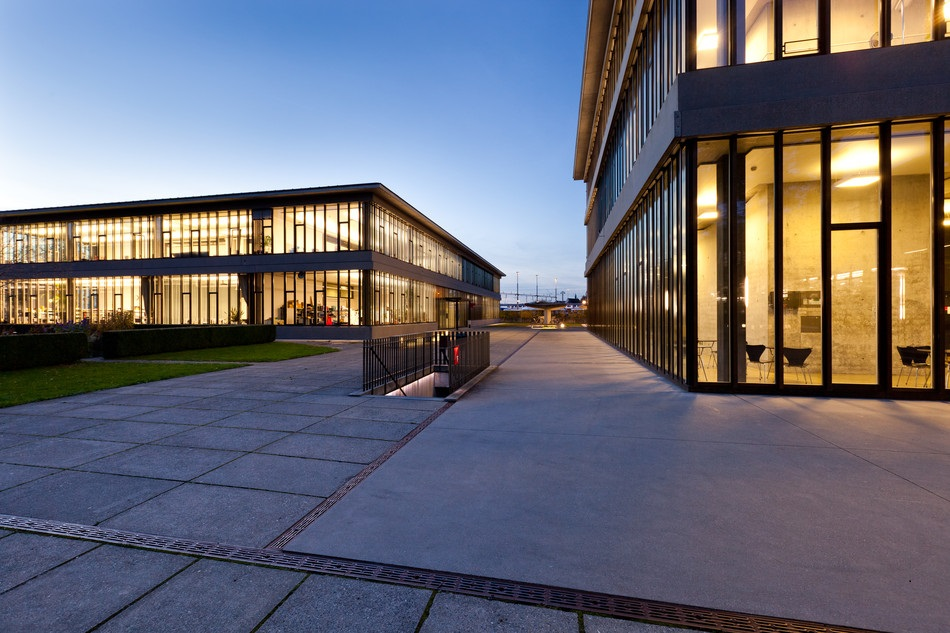
\includegraphics[width=10cm]{images/hsr}
            \nocite{titelbild}
        \end{center}
    
    	\begin{adjustwidth}{35mm}{40mm}	
   			\vfill
   			\large
            \textsf{\textbf{Autoren}}\\
            \null\hspace{0.01cm} \begin{tabular}{lll}
                \textsf{\AuthorOne} & \qquad & \textsf{\MatrikelOne}\\
                \textsf{\AuthorTwo} & \qquad & \textsf{\MatrikelTwo}\\
            \end{tabular}\\
   			\textsf{\textbf{Dozent}}\\
   			\null\quad\textsf{\Prof}\\
   			\textsf{\textbf{Betreuer}}\\
   			\null\quad\textsf{\Betreuer}\\
   			\textsf{\textbf{Modul}}\\
   			\null\quad\textsf{\Modul}\\
   			\hfill\hbox{}\\
            \textsf{
            \begin{tabular}{lll}
                \textbf{Version:}&\quad&\Version\\
                \textbf{Erstellt am:}&\quad&\ErstellDatum\\
                \textbf{Letzte Änderung am:}&\quad&\today\\
            \end{tabular}
            }\\
           	\hfill\hbox{}\\
               	\hfill\hbox{}\\
            \textsf{HSR Hochschule für Technik Rapperswil}\\
            \vspace{2cm}
   		\end{adjustwidth}		
	\end{adjustwidth}
\end{titlepage}
